\section{Design}
We've expanded the program to handle multiple neighbours,
to achieve this we've added a
\begin{lstlisting}
neighbour
\end{lstlisting}
struct which contains

% WEEEE

The original design of the system was designed for two hosts to communicate reliably with each other. To expand on this system, the information associated with a neighbour needed to exist in one instance per neighbour. The neighbours are stored in an array of structs for ease and in order encapsulate the information associated with a neighbour.\\
Furthermore, a central component in multiway communication is a means of distinguishing which neighbour is which. As the stations on the subnet already have unique IDs, these IDs can be used to uniquely identify the neighbours in a linear time lookup, which has a simple implementation for arrays, and won't take significant time for the array sizes being used. These station IDs are only used by the functions for which they are relevant though, as the general means of access for neighbour data are the array indices.\\
\\
Original setup
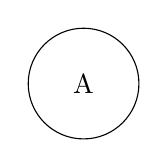
\begin{tikzpicture}

\draw[black] (0,0) circle (20pt) node [anchor=center] {A};

\end{tikzpicture}
